
\chapter{Problématiques}\label{ch:problematic}

\minitoc{}
\bigskip

% Spécifier la convergence
% deux pairs qui observe les mêmes effets d'opérations convergent
% Ici on parle d'op locales, elles peuvent être synchronisées de différentes
% manières.
% L'idée est de se centrer sur la confluence et de se déplacer au niveau de
% la couche réseau.

%La production collective de contenus par plusieurs centaines, voire plusieurs milliers d'utilisateur·ice·s est aujourd'hui une réalité.
%Par exemple, au sein des réseaux sociaux, des milliers d'utilisateur·ice·s réagissent en direct à des évènements et co-organisent des évènements.
%Cependant, la diffusion des activités massives de collaboration reste encore restreinte.
%Cette diffusion se heurte aux limitations conceptuelles des applications et des outils actuels de collaboration.
%Ces limitations sont induites par les infrastructures de collaboration sur lesquelles ils reposent.

Les infrastructures pair-à-pair de collaboration supportent les activités massives de collaboration.
Elles tolèrent les latences, les pannes, ainsi que les partitions réseaux.
Les collaborateur·ice·s peuvent modifier le contenu partagé de manière isolée.
Des collaborateur·ice·s géographiquement éloigné·e·s ou avec des connexions réseaux lentes et peu fiables peuvent contribuer à une collaboration.
Ces infrastructures sont donc bien adaptées à des collaboration qui impliquent des appareils mobiles.
Pour autant, elles assurent des latences basses lorsque les connexions réseaux le permettent.
Les collaborateur·ice·s ont donc l'illusion d'observer les modifications en temps réel lorsqu'elles et ils modifient simultanément un contenu.
Ces caractéristiques permettent de passer à l'échelle et de respecter le rythme de vie, ainsi que la manière de collaborer de chaque collaborateur·ice.

Pour ce faire, les infrastructures pair-à-pair de collaboration reposent sur la \emph{réplication optimiste}~\autocite{saito_2005_optimisticreplication}.
Chaque collaborateur·ice est associé·e à un pair qui possède une copie du contenu partagé.
Un pair interroge et modifie sa copie indépendemment des autres pairs.
En d'autres termes, les pairs n'ont pas besoin de se coordonner.
La copie est donc \emph{toujours disponible}~\autocite{mahajan_2011_cac} pour être interrogée ou modifiée. % par son/sa collaborateurice
C'est ce qui permet de tolérer les latences et les partitions réseaux.
La modification parallèle des copies conduit inévitablement à leur divergence~: les copies fournissent des réponses distinctes à une ou plusieurs interrogations qui peuvent leur être soumis.
Les pairs échangent à terme leurs modifications.
Les algorithmes de réplication de données sont en charge de la convergence des copies.
Ils doivent s'assurer qu'à terme les copies répondent de manière identique à toutes les interrogations qui peuvent leur être soumit.

La convergence des copies conditionne le succès d'une collaboration.
Si les collaborateur·ice·s ne sont pas capable de partager une vue globalement convergente dans des délais raisonnables, leur collaboration est probablement compromise.
Assurer à terme la convergence des copies est donc important.

Les algorithmes existants de réplication optimiste supposent généralement l'absence de pairs mal-intentionnés.
Plus largement, ils supposent l'absence d'un adversaire actif.
Cette hypothèse n'est pas réaliste au sein d'activités massives de collaboration.
Les pairs mal-intentionnés peuvent mener des attaques pour assurer une divergence permanente des pairs honnêtes.
Ils peuvent ainsi compromettre des collaborations.
Dans ce manuscrit de thèse, nous nous intéressons à cette problématique et nous proposons des mécanismes pour assurer à terme la convergence en présence d'un adversaire actif.

Ce chapitre introduit dans un premier temps la réplication de données. Il développe ensuite la notion de convergence et d'intention des opérations.
Il termine sur le modèle du système auquel nous nous intéressons et il définit l'adversaire du système.

\section{Réplication de données}\label{sec:optimistic-replication}

La réplication de données maintient des copies de contenus partagés sur un ensemble de pairs.
Elle augmente la disponibilité d'un contenu en permettant son interrogation et sa modification en dépit de la défaillance de pairs.
Les répliques sont souvent géographiquement réparties.
Ce qui rapproche les données des utilisateur·ice·s.
Elle réduit donc les latences pour interroger les contenus partagés.

Comparé à un contenu non-répliqué, un contenu répliqué a un nombre étendu de comportements.
Par exemple, des collaborateur·ice·s distinct·e·s peuvent modifier des copies distinctes d'un contenu répliqué.
Ces nouveaux comportements peuvent engendrer des scénarios difficiles à prévoir et traiter.
Idéalement, l'interrogation et la modification d'un contenu répliqué devrait se comporter comme si il existait une seule copie.
Dans ce cas, nous disons que le contenu partagé est \emph{fortement cohérent} et nous parlons de réplication pessimiste de données~\autocite{saito_2005_optimisticreplication}.
La~\autoref{fig:strong-consistency} met en évidence que l'interrogation d'un contenu fortement cohérent prend toujours en compte toutes les modifications précédemment effectuées.

\begin{figure}[htb]
\newcommand*\hsep{2.2}
\newcommand*\vsep{-1.4}
\centering
\begin{subfigure}{\linewidth}
    \centering
    \begin{tikzpicture}
        % Peers
        \node(A) at (0,0) {$p_A$};
        \node(B) at (0,\vsep) {$p_B$};
        \node (C) at (0,2*\vsep) {$p_C$};
        % Events
        \path (A)
            to +(\hsep,0) node[
                label=above:{$\trm{add}(1)$}
            ] (a2) {$\bullet$}
            to +(5*\hsep,0) node (aend) {}
        ;
        \path (B)
            to +(2*\hsep,0) node[
                label=above:{$\trm{rd}\set*{1}$}
            ] (b2){$\bullet$}
            to +(4*\hsep,0) node[
                label=above:{$\trm{rd}\set*{1,2}$}
            ] (b3){$\bullet$}
            to +(5*\hsep,0) node (bend) {}
        ;
        \path (C)
            to +(3*\hsep,0) node[
                label=above:{$\trm{add}(2)$}
            ] (c2) {$\bullet$}
            to +(5*\hsep,0) node (cend) {}
        ;
        % Timeline
        \foreach \src/\dest in {A/a2,B/b2,b2/b3,C/c2,a2/aend,b3/bend,c2/cend}
            \draw[timeline] (\src) to (\dest);
    \end{tikzpicture}
    \caption{}\label{subfig:strong-consistency-trace}
\end{subfigure}
\par\medskip
\begin{subfigure}{\linewidth}
    \centering
    \begin{tikzpicture}
        % Peers
        %\node (space) at (0,1.6) {};
        \node (V) at (0,0) {$p_V$};
        % Events
        \path (V)
            to +(\hsep,0) node[
                label=above:{$\trm{add}(1)$}
            ] (v2) {$\bullet$}
            to +(2*\hsep,0) node[
                label=above:{$\trm{rd}\set*{1}$}
            ] (v3){$\bullet {\scriptstyle}$}
            to +(3*\hsep,0) node[
                label=above:{$\trm{add}(2)$}
            ] (v4) {$\bullet {\scriptstyle}$}
            to +(4*\hsep,0) node[
                label=above:{$\trm{rd}\set*{1,2}$}
            ] (v5){$\bullet {\scriptstyle}$}
            to +(5*\hsep,0) node (vend) {}
        ;
        % Timeline
        \foreach \src/\dest in {V/v2,v2/v3,v3/v4,v4/v5,v5/vend}
            \draw[timeline] (\src) to (\dest);
    \end{tikzpicture}
    \caption{}\label{subfig:strong-consistency-single-copy}
\end{subfigure}
%
\caption[Réplication pessimiste d'un ensemble]{\subref{subfig:strong-consistency-trace} Histoire de l'exécution d'un ensemble répliqué fortement cohérent.
L'ensemble répliqué supporte une opération de modification $\set*{\trm{add}(n) \given n \in \mathbb{N}_0}$ qui ajoute un entier dans l'ensemble, et une opération d'interrogation $\trm{rd}$ qui donne la composition de l'ensemble.
Ainsi l'exécution de l'opération $\trm{add}(1)$ ajoute l'entier $1$ à l'ensemble, et nous notons $\trm{rd} \set*{1}$ une opération de lecture suivit de la valeur retournée par son exécution.
L'ensemble est initialement vide.
Le pair $p_A$ ajoute l'entier $1$.
Ultérieurement le pair $p_C$ ajoute l'entier $2$.
Le pair $p_B$ interroge à deux reprises l'ensemble.
Sa première interrogation se déroule entre les deux ajouts.
La seconde interrogation se déroule après les deux ajouts.
L'ensemble est fortement cohérent, une modification qui survient avant une autre modification ou une interrogation est donc visible à cette dernière.
La première interrogation retourne un singleton composé de l'élément $1$ et la seconde interrogation retourne un ensemble composé des éléments $1$ et $2$.
La cohérence forte maintient l'illusion de l'interrogation et la modification d'une seule copie.
\subref{subfig:strong-consistency-single-copy} L'histoire de l'exécution de cette copie abstraite peut être obtenue en projetant toutes les opérations sur un pair abstrait $p_V$.
}\label{fig:strong-consistency}
\end{figure}

Le maintien de l'illusion de l'interrogation et de la modification d'une seule copie a un coût.
Elle requiert une coordination étroite entre les pairs.
Une coordination qui peut se traduire par des communications systématiques avant chaque modification, voire avant chaque interrogation.
Les latences et les défaillances inhérentes aux réseaux~\cite{rotem_falalcies_2006} rendent cette coordination problématique.
Elle engendre plusieurs problèmes~:

\begin{description}
    \item[Disponibilité.] Le contenu ne peut plus être modifié, voire interrogé, lorsque des pairs sont isolés par des partitions réseaux.
    \item[Latence.] L'interrogation et la modification du contenu partagé est sujet aux latences du réseau et des pairs.
    La lenteur d'un pair ou d'une connexion réseau peut donc affecter l'ensemble du système.
    \item[Passage à l'échelle.] L'ajout de pairs, et donc de copies, peut détériorer la disponibilité et les latences étant donné que le nombre de pairs impliqués dans une coordination augmente.
\end{description}

Le théorème CAP~\cite{brewer_cap_2000,gilbert_cap_2002} montre l'impossibilité de garantir à la fois une cohérence forte et une disponibilité à tout moment en présence de partitions réseaux.
Nous pouvons illustrer cette impossibilité en prenant l'exemple d'une bibliothèque municipale qui possède un système répliqué d'emprunts de livres.
Deux usagers souhaitent faire un emprunt.
Les usagers sont connecté·e·s à des pairs distincts.
Supposons que le réseau est momentanément partitionné de telle manière à ce que les pairs considérés se trouvent dans l'impossibilité de communiquer.
Le système doit faire le choix entre le maintien d'une cohérence forte des emprunts ou la disponibilité d'emprunter.
Le maintien de la cohérence forte empêche tout emprunt tant que les partitions réseaux persistent.
La disponibilité d'emprunter en dépit du partitionnement peut conduire à des conflits.
Par exemple, des usagers peuvent effectuer des emprunts sur la même période d'un livre disponible en un seul exemplaire.

L'illustration proposée pourrait nous amener à penser que la cohérence forte peut être difficilement sacrifiée au bénéfice de la disponibilité.
En effet, le risque d'emprunts conflictuels pourrait produire des situations désagréables pour les usagers et la bibliothèque.
L'illustration proposée souffre du problème de la \emph{double-dépense}~\cite{chohan_doublespending_2017}.
L'emprunt d'un exemplaire d'un livre sur une période donnée correspond à une ressource consommable.
Cette ressource ne peut pas être consommée (dépensée) deux fois.
Ce problème n'est pas toujours rencontré.
Par exemple, un système de pétition en ligne ne souffre pas du problème de la \emph{double-dépense}.
Plusieurs personnes peuvent signer une pétition sans avoir besoin de se coordonner.

Les applications n'ont pas toujours besoin de maintenir une cohérence forte.
En général, le maintien d'une cohérence plus faible est suffisant~\autocite{terry_baseball_2013, hellerstein_calm_2019, decandia_dynamo_2007}.
Prenant cette observation en considération, la \textbf{réplication optimiste}~\autocite{saito_2005_optimisticreplication} sacrifie la cohérence forte pour atteindre une haute disponibilité et des latences basses.
Elle autorise la modification et l'interrogation des copies sans aucune coordination.
Les pairs modifient indépendemment leurs copies et échangeant leurs modifications ultérieurement.
Ce qui conduit à la divergence des copies et à l'intégration des modifications dans des ordres différents.
Deux copies divergentes fournissent des réponses différentes à au moins une interrogation.
La~\autoref{fig:optimistic-replication} illustre un scénario de réplication optimiste.

\begin{figure}[htb]
\newcommand*\hsep{2.2}
\newcommand*\vsep{-1.4}
\centering
\begin{tikzpicture}
    % Peers
    \node(A) at (0,0) {$p_A$};
    \node (B) at (0,\vsep) {$p_B$};
    % Event streams
    \path (A)
        to +(\hsep,0) node[
            label=above:{$\trm{add}(1)$}
        ] (a2) {$\bullet$}
        to +(2*\hsep,0) node[
            label=above:{$\trm{rd}\set*{1}$}
        ] (a3) {$\bullet$}
        to +(3*\hsep,0) node (a4) {$\bullet$}
        to +(4*\hsep,0) node (a5) {$\bullet$}
        to +(5*\hsep,0) node[
            label=above:{$\trm{rd}\set*{1,2}$}
        ] (a6) {$\bullet$}
        to +(6*\hsep,0) node (aend) {}
    ;
    \path (B)
        to +(\hsep,0) node[
            label=below:{$\trm{add}(2)$}
        ] (b2) {$\bullet$}
        to +(2*\hsep,0) node[
            label=below:{$\trm{rd}\set*{2}$}
        ] (b3) {$\bullet$}
        to +(3*\hsep,0) node (b4) {$\bullet$}
        to +(4*\hsep,0) node (b5) {$\bullet$}
        to +(5*\hsep,0) node[
            label=below:{$\trm{rd}\set*{1,2}$}
        ] (b6){$\bullet$}
        to +(6*\hsep,0) node (bend) {}
    ;
    % hb
    \foreach \src/\dest in {A/a2,a2/a3,a3/a4,a4/a5,a5/a6,B/b2,b2/b3,b3/b4,b4/b5,b5/b6,a6/aend,b6/bend}
        \draw[timeline] (\src) to (\dest);
    \draw[hb] (b4) to (a5);
    \draw[hb] (a4) to node[fill=white]{\footnotesize sync} (b5);
\end{tikzpicture}
\caption[Réplication optimiste d'un ensemble]{Exemple de réplication optimiste d'un ensemble.
Les pairs $p_A$ et $p_B$ débutent avec un ensemble vide.
$p_A$ ajoute l'élément $1$ sur sa copie.
$p_B$ ajoute en parallèle l'élément $2$ sur sa copie.
Les copies divergent~: les deux pairs obtiennent des singletons distincts.
Ils synchronisent ultérieurement leurs copies pour échanger et intégrer leurs modifications respectives.
Les modifications ne sont pas intégrés dans le même ordre sur les copies~: ils intégrèrent la modification de l'autre pair après avoir intégré leur propre modification.
Les copies finissent par converger~: les pairs obtiennent le même ensemble.}\label{fig:optimistic-replication}
\end{figure}

Plusieurs modèles de cohérence dits \enquote{faibles} peuvent être respectés par un protocole de réplication optimiste.
L'une des garanties élémentaires de ces modèle concerne la convergence des copies.
En l'absence de modifications, les copies devraient converger.
Toute interrogation sur deux copies convergentes devraient donner les mêmes réponses.
La convergence peut être définit de différentes manières.
La \emph{cohérence à terme}~\autocite{terry_sessionguarentees_1994,saito_2005_optimisticreplication, vogels_eventuallyconsistent_2009} offre la garantie de convergence la plus faible qu'un protocole de réplication optimiste doit respecter.
Elle garantit que deux copies finissent par converger dès lors qu'elles ont intégré le même ensemble de modifications.
Elle garantit également qu'une modification intégrée par un pair finit par l'être par les autres pairs.

\begin{definition}[Cohérence à terme]\label{def:eventual-consistency}
  Une exécution qui respecte la cohérence à terme, respecte les propriétés suivantes~:
  \begin{description}
  \item[\namedlabel{itm:ec1}{EC1} (intégration à terme)] Une modification intégrée sur la copie d'un pair est à terme intégrée par l'ensemble des pairs.
  \item[\namedlabel{itm:ec2}{EC2} (convergence à terme)] Les pairs qui ont intégrés le même ensemble de modifications ont des copies qui convergent à terme.
  \end{description}
\end{definition}

Le fait que la cohérence à terme offre une garantie de convergence si faible suggère que la tâche est difficile.
Cette difficulté réside principalement dans la présence de conflits de modification.
La~\autoref{fig:modif-conflict} présente un scénario où un conflit de modification survient.
La réplication optimiste fait l'hypothèse \textquote{optimiste} que les conflits de modification sont rares et peuvent être résolu ultérieurement.
Les pairs doivent donc gérer les conflits de modification et se mettre d'accord sur un moyen de les résoudre.
Dans la~\autoref{sec:convergence}, nous nous intéressons aux différentes garanties qui peuvent contraindre la convergence et donc la manière de résoudre les conflits de modification.

\begin{figure}[htb]
\newcommand*\hsep{2.2}
\newcommand*\vsep{-1.4}
\centering
\begin{tikzpicture}
    % Peers
    \node(A) at (0,0) {$p_A$};
    \node (B) at (0,\vsep) {$p_B$};
    % Event streams
    \path (A)
        to +(\hsep,0) node[
            label=above:{$\trm{add}(1)$}
        ] (a2) {$\bullet$}
        to +(2*\hsep,0) node[
            label=above:{$\trm{rmv}(1)$}
        ] (a3) {$\bullet$}
        to +(3*\hsep,0) node[
            label=above:{$\trm{rd}\emptyset$}
        ] (a4) {$\bullet$}
        to +(4*\hsep,0) node (a5) {$\bullet$}
        to +(5*\hsep,0) node (a6) {$\bullet$}
        to +(6*\hsep,0) node[
            label=above:{$\trm{rd}\set*{1}$}
        ] (a7) {$\bullet$}
        to +(7*\hsep,0) node (aend) {}
    ;
    \path (B)
        to +(\hsep,0) node[
            label=below:{$\trm{add}(1)$}
        ] (b2) {$\bullet$}
        to +(3*\hsep,0) node[
            label=below:{$\trm{rd}\set*{1}$}
        ] (b3) {$\bullet$}
        to +(4*\hsep,0) node (b4) {$\bullet$}
        to +(5*\hsep,0) node (b5) {$\bullet$}
        to +(6*\hsep,0) node[
            label=below:{$\trm{rd}\emptyset$}
        ] (b6){$\bullet$}
        to +(7*\hsep,0) node (bend) {}
    ;
    % Timeline
    \foreach \src/\dest in {A/a2,a2/a3,a3/a4,a4/a5,a5/a6,a6/a7,B/b2,b2/b3,b3/b4,b4/b5,b5/b6,a6/aend,b6/bend}
        \draw[timeline] (\src) to (\dest);
    \draw[hb] (b4) to (a6);
    \draw[hb] (a5) to node[fill=white]{\footnotesize sync} (b5);
\end{tikzpicture}
\caption[Conflit de modification d'un ensemble répliqué]{Exemple de conflit de modification.
Les pairs $p_A$ et $p_B$ répliquent un ensemble qui supporte une opération d'ajout $\set*{\trm{add}(n) \given n \in \mathbb{N}_0}$, une opération de suppression $\set*{\trm{rmv}(n) \given n \in \mathbb{N}_0}$, et une opération de lecture $\trm{rd}$.
$p_A$ ajoute l'élément $1$ puis le supprime. En parallèle, $p_B$ ajoute également l'élément $1$.
L'ajout et la suppression en parallèle d'un même élément constitue un conflit de modification.
L'élément ne peut pas être à la fois présent et absent de l'ensemble.
L'intégration \textquote{naïve} des modifications dans des ordres distincts conduit à une divergence des copies.}\label{fig:modif-conflict}
\end{figure}


\section{Convergence des copies}\label{sec:convergence}

% coordination -> perf en baisse
% perf en baisse -> moins bonne vivacité ?
% Contraindre plus la convergence pour meilleur vivacité.

% Rappeler que les coordinations sont facteurs de lenteurs ?

Un protocole de réplication optimiste autorise les modifications en concurrence sans coordination.
La divergence des copies est donc inévitable.
Le succès d'une collaboration est conditionné par la capacité des copies à converger.
\textcite{ignat_2015_user-and-delay} ont montré que les activités de collaboration en simultané étaient compromises lorsque le délai entre des modifications de contenu et leurs observations par les autres était trop important.
Dans l'idéal la convergence devrait être atteinte le plus rapidement possible.
Pour réduire au maximum les délais de convergence, toutes coordinations devrait être évitées~\autocite{bailis_coordavoidance_2014}.

\begin{figure}[htb]
\newcommand*\hsep{1.7}
\newcommand*\vsep{-1.4}
\centering
\begin{tikzpicture}
    % Peers
    \node(A) at (0,0) {$p_A$};
    \node (B) at (0,\vsep) {$p_B$};
    % Events
    \path (A)
        to +(\hsep,0) node[
            label=above:{$\trm{add}(1)$}
        ] (a2) {$\bullet$}
        to +(2*\hsep,0) node[
            label=above:{$\trm{rmv}(1)$}
        ] (a3) {$\bullet$}

        to +(3*\hsep,0) node (a4) {$\bullet$}
        to +(4*\hsep,0) node (a5) {$\bullet$}
        to +(5*\hsep,0) node[
            label=above:{$\trm{rd}\set*{1}$}
        ] (a6) {$\bullet$}
        to +(8*\hsep,0) node[
            label=above:{$\trm{rd}\set*{1}$}
        ] (a7) {$\bullet$}
        to +(9*\hsep,0) node (aend) {}
    ;
    \path (B)
        to +(\hsep,0) node[
            label=below:{$\trm{add}(1)$}
        ] (b2) {$\bullet$}

        to +(3*\hsep,0) node (b3) {$\bullet$}
        to +(4*\hsep,0) node (b4) {$\bullet$}
        to +(5*\hsep,0) node[
            label=below:{$\trm{rd}\emptyset$}
        ] (b5){$\bullet$}
        to +(8*\hsep,0) node[
            label=below:{$\trm{rd}\set*{1}$}
        ] (b6){$\bullet$}
        to +(9*\hsep,0) node (bend) {}
    ;
    % Coordinations
    \path (A)
        to ++(6*\hsep,1) coordinate (coord1)
        to node[above,midway,
            label=above:{coordination}
        ]{} +(\hsep,0);
    % Timelines
    \foreach \src/\dest in {A/a2,a2/a3,a3/a4,a4/a5,a5/a6,a6/a7,B/b2,b2/b3,b3/b4,b4/b5,b5/b6,a6/aend,b6/bend}
        \draw[timeline] (\src) to (\dest);
    % Coordination
    \draw[fill=white] (coord1) rectangle +(\hsep,-2+\vsep);
    % Sync
    \draw (b3) edge[hb] (a5);
    \draw (a4) edge[hb] node[fill=white]{\footnotesize sync} (b4);
\end{tikzpicture}
\caption[Réplication optimiste et coordination]{Exemple de coordination après l'intégration de modifications.
Les pairs $p_A$ et $p_B$ intègrent les modifications de chacun.
Les copies ne convergent pas.
Les pairs se coordonnent après l'intégration des modifications afin de converger.}\label{fig:convergence-post-coord}
\end{figure}


Un protocole de réplication optimiste garantit une \emph{convergence à terme} des copies des pairs.
La convergence à terme assure seulement que les pairs qui ont intégrés un même ensemble de modification convergeront dans un futur plus ou moins proche.
Elle ne donne aucune borne sur le temps nécessaire et le nombre de communications nécessaires  pour converger.
La \autoref{fig:convergence-post-coord} illustre un scénario dans lequel deux pairs intègrent leurs modifications respectives et se coordonnent ensuite afin de converger.

Cette propriété de convergence est faible car il s'agit d'une propriété de vivacité.
Une propriété de vivacité peut être violée en plusieurs points de l'exécution d'un protocole~\autocite{alpern_liveness_1985}.
Elle décrit \enquote{quelque chose de positif} qui devrait survenir.
La formulation d'une propriété de vivacité inclut généralement l'expression \enquote{à terme}.

Afin de faire converger plus rapidement les copies et exclure l'utilisation de coordinations, nous devons contraindre la convergence avec des propriétés de sûreté.
Une propriété de sûreté décrit \enquote{quelque chose de mauvais} qui ne devrait jamais survenir.
Une propriété de sûreté doit être respectée en tout point de l'exécution d'un protocole.
\textcite{shapiro_2011_crdt} proposent la \emph{convergence forte} comme propriété de sûreté de la convergence.

\begin{definition}[Convergence forte]\label{def:strong-convergence}
Les pairs qui ont intégré le même ensemble de modifications ont des copies convergentes.
\end{definition}

La \emph{convergence forte} ne nécessite pas de coordinations après l'intégration des modifications.
Cependant, elle n'exclut pas l'utilisation de coordination avant l'intégration des modifications.
Les pairs peuvent décider d'un moyen de résoudre les éventuels conflits de modification.
Par exemple, un protocole peut utiliser un pair privilégié qui ordonne les modifications selon un ordre global~\autocite{terry_bayou_1995}.
\textcite{mahajan_2011_cac} proposent la \emph{convergence unidirectionelle} pour éviter toutes coordinations.
L'idée centrale de la \emph{convergence unidirectionelle} est que deux pairs $p_A$ et $p_B$ devraient être capable de faire converger leur copie en deux étapes de communication unidirectionelle~: $p_A$ envoie des modifications à $p_B$, puis $p_B$ envoie des modifications à $p_A$.

%\begin{definition}[Convergence partielle]\label{def:partial-convergence}
%$p_A$ \emph{converge partiellement} avec $p_B$ si et seulement si il suffit que
%\begin{enumerate}[label=(\roman*)]
%\item $p_A$ et $p_B$ arrêtent de modifier leur copie et de communiquer avec les autres pairs
%\item $p_B$ transmette à $p_A$ les modifications qu'il a intégré et $p_A$ intègre ces dernières
%\end{enumerate}
%pour que les copies de $p_A$ et $p_B$ convergent.
%\end{definition}
%
%\begin{definition}[Convergence unidirectionelle]\label{def:one-way-convergence}
%Pour tout pair $p_A$ qui arrête de modifier sa copie et de communiquer avec tout pair, il suffit que $p_A$ transmette à $p_B$ les modifications qu'il a intégré et que $p_B$ intègre ces dernières pour que $p_A$ \emph{converge partiellement} avec $p_B$.
%\end{definition}
%
%\vicnote{Y-a t-il un intérêt à renforcer cette propriété ? Non... => supprimer ce qui arrive après ?}
%
%Nous pouvons renforcer cette propriété en exigeant que deux pairs $p_A$ et $p_B$ soient capable de converger en initiant deux communications unidirectionnelles en concurrence~: $p_A$ envoie des modifications à $p_B$, et $p_B$ envoie en parallèle des modifications à $p_A$.
%
%\begin{definition}[Convergence unidirectionelle forte]\label{def:strong-one-way-convergence}
%Si $p_A$ et $p_B$ arrêtent de modifier leur copie et arrêtent de communiquer avec les autres pairs, alors il suffit que
%\begin{enumerate}[label=(\roman*)]
%\item $p_A$ transmette à $p_B$ les modifications qu'il a intégré
%\item $p_B$ transmette (éventuellement en parallèle) à $p_A$ les modifications qu'il a intégré
%\item $p_A$ et $p_B$ intègrent (éventuellement en parallèle) les modifications qu'ils ont reçu de chacun
%\end{enumerate}
%pour que leurs copies convergent.
%\end{definition}

La non-nécessité de coordination pour obtenir des copies convergentes, suggère une résolution déterministe des conflits de modification.
Dans le cas de la bibliothèque, on peut supposer que dans la majorité des cas des emprunts simultanés concernent des livres ou des exemplaires différents sur des périodes distinctes.
Toutefois, des conflits d'emprunts peuvent survenir.
Le nombre d'exemplaires d'un nouveau livre peut être insuffisant par rapport au nombre de lecteur·ice·s intéressé·e·s.
Plusieurs stratégies peuvent être mises en place pour résoudre ces conflits.
On peut considérer que l'emprunteur·ice final·e correspond à la personne qui a fait l'emprunt en premier.

%Au fil des modifications et de leurs échanges, les pairs suivent des cycles de divergence et de convergence.


% \section{Intention des opérations}

% Il peut exister plusieurs manière de réconcilier les copies d'un contenu partagé.
% Dans la \autoref{fig:optimistic-replication}, les pairs intègrent les ajouts de chaque pair afin de converger vers un état équivalent.
% Cependant, rien n'empêche de réconcilier les copies en rejetant les ajouts effectuées en parallèle.
% Les pairs $p_A$ et $p_B$ pourraient ainsi converger vers un ensemble vide.

% Cette approche de réconciliation pourrait surprendre les collaborateur·ice·s.
% En effet, si deux éléments sont ajoutés en parallèle dans l'ensemble, on pourrait s'attendre à ce qu'ils appartiennent dans l'ensemble après la réconciliation des copies.
% \textcite{sun_1998_cci} parlent d'intention des opérations.
% Intuitivement, l'intention d'une opération capture l'effet observable de l'opération.
% Cette effet devrait être observable quelque soit le pair qui exécute l'opération.

% L'intégration d'opération concurrentes ou plus largement la réconciliation de copies devrait préserver autant que possible l'intention des opérations qui sont exécutées.
% L'intention d'une opération peut être exprimée comme une postcondition.
% Cette postcondition doit être prudemment spécifiée afin d'assurer son respect quelque soit l'ordre d'exécution des opérations qui sont indépendantes de l'opération considérée.
% Les opérations indépendantes correspondent aux opérations concurrentes et éventuellement à d'autres opérations.

% Reprenons l'exemple de l'ensemble répliqué pour illustrer la spécification de l'intention des opérations.
% Le type abstrait de donnée Ensemble spécifie l'ajout d'un élément dans un ensemble comme l'ensemble auquel a été ajouté l'élément.
% Dans un premier temps nous pouvons définir l'intention de l'ajout d'un élément comme sa spécification.
% Dans la \autoref{fig:optimistic-replication} l'opération $\trm{add}(1)$ a comme intention l'obtention du singleton $\set*{1}$.
% L'opération $\trm{add}(2)$ a comme intention l'obtention du singleton $\set*{2}$.
% La réconciliation des copies des deux pairs conduit nécessairement à la violation de l'intention de l'une des opérations.
% Nous pouvons définir plus prudemment l'intention des opérations de telle manière à ce qu'elle offre une garantie pertinente tout en évitant leur violation.
% Dans notre cas, nous pouvons définir l'intention d'un ajout comme l'obtention d'un ensemble qui contient à la fois l'élément ajouté et les éléments précédemment ajoutés.
% La présence d'éléments ajoutés en concurrence n'est donc pas exclut.
% Dans la \autoref{fig:optimistic-replication} l'opération $\trm{add}(1)$ a comme intention l'obtention d'un ensemble qui contient l'élément $1$.
% L'opération $\trm{add}(2)$ a comme intention l'obtention d'un ensemble qui contient l'élément $2$.

% % Intention -> No rollbacks
% La préservation de l'intention des opérations peut plus largement retranscrire le principe d'intégrer les opérations de chaque pair sans les ignorer.
% Ce qui empêche la mise en place de retour en arrière.


\section{Modèle du système}

\vicnote{Figure à mettre à jour}

\begin{figure}[htb]
\centering
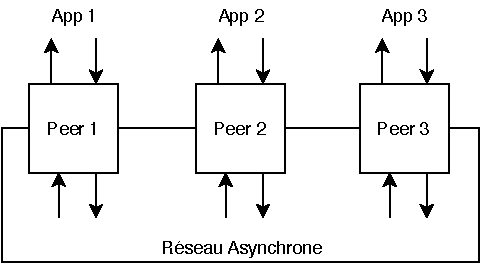
\includegraphics{fig/impl.pdf}
\caption{Une infrastructure de collaboration composée de 3 pairs qui répliquent le contenu partagé. Les 3 pairs sont connectés par un réseau asynchrone.}\label{fig:collab-system}
\end{figure}

Dans les infrastructure pair-à-pair de collaboration, chaque collaborateur·ice est associé·e à un pair qui lui est exclusif.
\textcite{guerraoui_2016_tradeoffs-replication} parlent de \emph{sticky availability}.
L'une des principales implications est que des pairs peuvent joindre et quitter le système de réplication au gré des connexions et des déconnexions des collaborateur·ice·s.
De nouveaux pairs peuvent joindre lorsque de nouveaux et nouvelles collaborateur·ice·s joignent le groupe
Des pairs existants peuvent se déconnecter indéfiniment lorsque les collaborateur·ice·s associé·e·s quittent le groupe.

Pour interroger et modifier le contenu partagé, un·e collaborateur·ice soumet des opérations au pair qui lui est associé.
Ces opérations dépendent du type du contenu répliqué.
Dans la~\autoref{fig:optimistic-replication}, l'ensemble répliqué peut être modifié par une opération d'ajout $\set*{\trm{add}(n) \given n \in \mathbb{N}_0}$ et peut être intérrogé par une opération de lecture $\trm{rd}$ qui donne la composition de l'ensemble.
Les opérations sont d'abord intégrées sur la copie que le pair détient.
Les pairs synchronisent leur copie en arrière plan.
Une synchronisation peut s'effectuer après chaque nouvelle modification ou peut être espacée dans le temps.

Nous supposons qu'un·e collaborateur·ice ne peut être dissocié·e du pair qui lui est attaché.
La copie est donc \emph{toujours disponible}~\autocite{mahajan_2011_cac} pour être interrogée et modifiée.


\section{Adversaire du système}

Un protocole de réplication optimiste doit respecté un ensemble de propriétés de cohérence.
Pour assurer ces propriétés, un protocole doit résister aux défaillances et aux comportements mal-intentionnés qu'il rencontre au cours de ses exécutions.
Par exemple, il doit se prémunir contre les défaillances inhérentes aux réseaux.

Les protocoles de réplication optimiste supposent généralement l'absence de comportements mal-intentionnés.
Cette hypothèse n'est pas réaliste au sein d'activités massives de collaboration.
Plus un groupe de collaborateur·ice·s est large plus il est probable que le groupe inclut un ou plusieurs utilisateur·ice·s mal-intentionné·e·s.

Les défaillances d'un système peuvent être accidentelles ou résultantes de comportements mal-intentionnés.
Sans perte de généralité, nous considérons que toute défaillance est le résultat de comportements mal-intentionnés.
Ces comportements sont exprimés par l'adversaire du système.
L'adversaire du système est mû par un objectif et contrôle des ressources, tels que le réseau et des pairs, pour atteindre son objectif.

L'objectif de notre adversaire est de compromettre la convergence des copies des collaborateur·ice·s honnêtes~\footnote{Dans la littérature le terme \textquote{correct} est également utilisé.}.
Et ce dans le but de faire échouer leur collaboration.
Pour simplifier les références ultérieures, nous proposons de classifier les capacités de l'adversaire à travers trois profils~: réseau asynchrone non-fiable, réseau corrompu, pairs perturbées, pairs mal-intentionnés.

\paragraph{Réseau asynchrone non-fiable.} L'adversaire contrôle le réseau et peut exposer l'ensemble des comportements observées sur un réseau asynchrone non-fiable~\autocite{lynch_1996_asyncnet}.
En particulier, les messages échangées entre les pairs peuvent être réordonnés, dupliqués, retardés, et omis.
L'adversaire peut séparer les pairs en partitions.
Toutefois il ne peut pas empêcher les pairs honnêtes de s'échanger à terme un nombre non-borné de messages.
Ce qui implique qu'il ne peut pas maintenir indéfiniment une partition réseau ou omettre tous les messages émit par un pair.
Cette limitation est nécessaire pour que des propriétés de vivacité, tel que l'\emph{intégration à terme}, soient réalisables.

\paragraph{Réseau asynchrone corrompu.} L'adversaire a les limitations et les capacités décrites dans le profil \emph{réseau asynchrone non-fiable}.
En outre, il peut contrefaire des messages.
Il peut par exemple changer l'émetteur d'un message ou le contenu d'un message.

\paragraph{Pairs restaurés.} L'adversaire peut perturber un pair honnête.
Il peut le soumettre à des lenteurs arbitraires.
Il ne peut toutefois pas empêcher un pair de progresser dans l'exécution du protocole.
L'adversaire peut également produire des pannes qui rend momentanément le pair indisponible.
Nous supposons que les pairs honnêtes disposent d'une mémoire durable et fiable de telle sorte à ce qu'ils retrouvent l'état dans lequel ils se trouvaient juste avant leur dernière panne.
Pour les mêmes raisons que celles évoqués dans le profil \emph{réseau asynchrone non-fiable}, l'adversaire ne peut pas provoquer des pannes dans l'objectif d'arrêter l'exécution définitive du protocole ou d'empêcher indéfiniment les pairs honnêtes de s'échanger un nombre non-borné de messages.

\paragraph{Pairs mal-intentionnés.} L'adversaire contrôle un ensemble de pairs mal-intentionnés~\footnote{Dans la littérature, le terme \textquote{défectueux} est également utilisé.} qui peuvent librement travailler de concert. Il peut librement connecter de nouvelles pairs mal-intentionnés et déconnecter, éventuellement indéfiniment, des pairs mal-intentionnés. Les pairs mal-intentionnés peuvent se comporter de manière arbitraire.

\paragraph{}L'adversaire peut utiliser l'ensemble de ses capacités et de ses ressources pour exprimer des comportements complexes.
Toutefois, nous supposons les limitations suivantes~:

\begin{itemize}
  \item L'adversaire a des ressources limitées en puissance de calcul et en temps.
  Ces ressources ne sont pas suffisantes pour compromette les primitives de cryptographies, telles que les signatures digitales et les fonctions de hachage résistants aux collisions.
  \item Il ne peut pas empêcher un pair honnête d'authentifier la clef publique d'un autre pair honnête.
  L'adversaire ne peut pas obtenir la clef privé d'un pair honnête et il ne peut donc pas usurper son identité cryptographique.
\end{itemize}

Les protocoles de réplication optimiste s'intéressent généralement à un adversaire qui a les profils \emph{réseau asynchrone non-fiable} et \emph{pairs restaurés}.
En ajoutant les deux autres profils \emph{réseau corrompu} et \emph{pairs mal-intentionnés} nous obtenons un adversaire qui est Byzantin~\autocite{lamport_1982_byzantinegeneralsproblem}.

Certain·e·s auteur·ice·s font la distinction entre les pairs mal-intentionnés et les pairs honnêtes-mais-défaillants.
Un pair honnête-mais-défaillant expose des comportements qui peuvent être prêtés à un pair mal-intentionné.
Un pair honnête n'a pas la capacité de décider si un comportement nuisible d'un pair est le résultat d'une défaillance ou de motivations mal-intentionnées.
Nous considérons donc les pairs honnêtes-mais-défaillants comme des pairs mal-intentionnés.


\section{Synthèse et objectifs}

Un protocole de réplication optimiste autorise la modification et l'interrogation des copies d'un contenu répliqué sans aucune coordination.
Les copies sont donc toujours disponible pour être modifiées et interrogées.
La modification concurrente des copies conduit inévitablement à leur divergence.
La convergence des copies est une propriété essentielle des infrastructures de collaboration.
Elle conditionne le succès d'une collaboration.
Afin d'assurer des latences faibles et un passage à l'échelle du protocole, nous nous intéressons à des propriétés de convergence qui ne nécessitent pas de coordination.

Le passage à l'échelle et les latences faibles des protocole de réplication optimiste auxquels nous nous intéressons permet le support de collaboration massive.
Ce type de collaboration à une probabilité plus importante de rencontrer des comportements mal-intentionnés.
Nous avons choisi de nous intéresser à des protocoles qui résistent à un adversaire Byzantin.
Ce dernier contrôle le réseau et un ensemble de pairs mal-intentionnés.
Il peut également perturber le fonctionnement des pairs honnêtes.

Dans ce manuscrit nous cherchons à assurer la convergence des copies des pairs honnêtes sans la nécessité de coordination.
